\documentclass[11pt]{article}
\renewcommand{\baselinestretch}{1.8}
\usepackage{textcomp}
\usepackage{fontenc}
\usepackage{graphicx}
\usepackage{caption} % for Fig. captions
\usepackage{gensymb} % for \degree
\usepackage{placeins} % for \images
\usepackage[margin=1in]{geometry} % to set margins
\usepackage{setspace}
\usepackage{lineno}
%\usepackage{cite}
\usepackage{amssymb} % for math symbols
\usepackage{amsmath} % for aligning equations
\usepackage[sort&compress]{natbib}
%\bibliographystyle{..//..//refs/styles/newphyto.bst}
\usepackage{xr-hyper}
\externaldocument{reconciling_FLS_SUPP_wbbl}
%\externaldocument{newphytrevresp_p2}
%\externaldocument{round2revresp_p2}
\linenumbers
% line numbers for letter
% line numbers for letter


\title{Reconciling competing hypotheses regarding flower-leaf sequences in temperate forests for fundamental and global change biology}
\date{}
\author{D.M. Buonaiuto $^{1,2,a}$, Ignacio Morales-Castilla$^{3}$, E.M. Wolkovich$^{4}$}

%3510 words
\begin{document}
\maketitle
\linenumbers
\noindent \emph{Author affiliations:}\\
\noindent $^1$Arnold Arboretum of Harvard University, Boston, Massachusetts, USA. ORCID: 0000-0003-4022-2591\\
$^2$Department of Organismic and Evolutionary Biology, Harvard University, Cambridge, Massachusetts, USA \\
$^3$Global Change Ecology and Evolution (GloCEE), Department of Life Sciences, University of Alcal\`a  28805, Alcal\`a de Henares, Spain. ORCID: 0000-0002-8570-9312\\
$^4$Forest \& Conservation Sciences, Faculty of Forestry, University of British Columbia, Vancouver, British Columbia, Canada\\
$^a$Corresponding author: 617.823.0687; dbuonaiuto@g.harvard.edu

\noindent \emph{Keywords:} deciduous forests, flower-leaf sequences, global change, hysteranthy, phenology, phylogeny \\ 
\emph{Paper type:} Viewpoint\\
\emph{Social media accounts:} Twitter: @TheHolbrookLab, @GloCEE\_EcoEvo.   

 \emph{Counts}: Words: Summary: 192; Main text: 3366; References: 48;  Figures: 4 (all color). Supporting Information: 8 supplemental figures, 1 supplemental table and Methods.
\newpage

\section*{Summary}
Phenology is a major component of an organism's fitness. While individual phenological events affect fitness, growing evidence suggests that the relationship between events may be equally or more important. This may explain why temperate deciduous woody plants exhibit considerable variation in the order of reproductive and vegetative events, or flower-leaf sequences (FLSs). There is evidence to suggest that FLSs may be adaptive\linelabel{small1.r2}, with several competing hypotheses to explain their function. Here, we advance existing hypotheses with a new framework that accounts for quantitative FLS variation at multiple taxonomic scales using case studies from temperate forests. Our inquiry provides several major insights towards a better understanding of FLS variation. First, we show that support for FLS hypotheses is sensitive to how FLSs are defined, with quantitative definitions being the most useful for robust hypothesis testing. Second, we demonstrate that concurrent support for multiple hypotheses should be starting point for future FLS analyses. Finally, we highlight how adopting a quantitative, intra-specific approach generates new avenues for evaluating fitness consequences of FLS variation and provides cascading benefits to improving predictions of how climate change will alter FLSs and thereby re-shape plant communities and ecosystems.

\section*{Introduction}
Phenology, the timing of seasonal life cycle events, allows organisms to synchronize their activity with optimum environmental conditions \citep{Forrest2010}. It is not only individual\linelabel{small1.r1} phenological stages that affect an organism's performance, but also their chronology \citep{Firmat2017,Vitasse2010,Ettinger2018}.\\

\noindent One phenological relationship that has long received scientific interest \citep[see][]{Robertson1895} and, recently, increased attention \citep[e.g.][]{Savage2019, Gougherty2018} is the flower-leaf phenological sequence (FLS) of temperate deciduous woody plants. In a typical model of plant life-history, vegetative growth precedes reproduction. However, for many species in the forests of Eastern North America (and other temperate regions of the Northern Hemisphere), it is not the green tips of new shoots that mark the commencement of the growing season, but the subtle colors of\linelabel{small2.r1} flowers. Previous work by \citet{Gougherty2018} found that as many as 30\% of tree species of the Midwestern United States flower prior to leafout\linelabel{small3.r1}. The prevalence of this FLS may be surprising as it requires plants to invest in reproduction from stored carbohydrates at a time when their reserves are at their lowest level \citep{Primack1987}\linelabel{tradeoff1}, but this trade-off suggests that flowering-first has some adaptive significance \citep{Rathcke_1985}\linelabel{smallx.r2}.\\

\noindent Understanding this phenological pattern is timely because anthropogenic climate change is altering FLSs. Long-term data shows that the number of days between flowering and leafout is increasing as a result of climate change, but the rate of change differs up to five-fold among species, with flowering-first species seemingly more sensitive \linelabel{ser1} to climate change (Fig. \ref{fig:climchange}). If FLSs are indeed an important component of woody plant fitness, this inter-specific variation will exacerbate fitness differences between species, influencing which species will persist under altered climate conditions.\\ 

\noindent Long-term datasets also demonstrate high within-species variability in FLSs.\linelabel{small4.r1} Despite recent advances in understanding the physiology and evolution of FLSs \citep{Gougherty2018,Savage2019}, most analyses have not directly addressed this variability---potentially slowing progress in predicting how FLSs will respond to climate change\linelabel{small5.r1}. While the literature provides some general correlations between flower and leaf phenology \citep[e.g.][]{Lechowicz_1995, Ettinger2018}, there have been few, if any, analyses of higher-resolution patterns \citep{Gougherty2018}. \\

\noindent We propose a new framework for the study of FLSs built on quantitative measures of both inter- and intra-specific FLS variation. This shift will improve predictions of how FLS patterns will change in the future, and  may reveal novel avenues to better understand the fundamental biology of this phenological sequence. Here we 1) review hypotheses of the function of FLS variation 2) evaluate the biological basis of the current categorical FLS framework and 3) present our proposed quantitative framework using a detailed case study of long-term phenology records from Harvard Forest in Petersham, MA.

\section*{Hypotheses for flower-leaf sequence variation}
\subsubsection*{ Wind pollination}
\noindent The most prevalent FLS hypothesis suggests that flowering-first is an adaptation for wind-pollination, with leafless flowering allowing for more efficient pollen transfer \citep{Whitehead1969}(Fig. \ref{fig:conceptual}a). The primary evidence for this hypothesis comes from pollen diffusion studies \citep[e.g., particle movement through closed and open canopies,][]{Niklas1985, Milleron2012} and suggests canopy structure encumbers pollen movement.
\subsubsection*{Water limitation}
\noindent Another hypothesis suggests that flowering before leaf development is an adaptation to reduce water stress caused by concurrently maintaining floral hydration and leaf transpiration \citep{Franklin2016} (Fig. \ref{fig:conceptual}b). Observations from the dry tropics, where this FLS is also common, confirm that the timing of flowering in many species is associated with a water status recovery due to leaf drop \citep{Borchert1983,Reich1984}, and that flower tissue is more sensitive to drought-induced xylem embolism\linelabel{hydro} than leaf tissue \citep{Zhang2017}. Despite the fact that temperate forests are rarely water-limited during the spring when flowering and leafing occur \citep{Polgar2011}, a recent analysis by \citet{Gougherty2018} found strong associations between flowering-first and water use traits for temperate species. This suggests that this hypothesis merits broader consideration and further development for the\linelabel{highlat} temperate zone as well (see Supporting Information \nameref{Methods S1}, ``The water limitation hypothesis in wet temperate forests"). 
 
\subsubsection*{Early flowering}
\noindent A third possibility is that the flowering-first FLS is a byproduct of selection for early flowering  (Fig. \ref{fig:conceptual}c). Flowering-first species are among the earliest in a community to flower seasonally, which may be an adaptation to accommodate later phenological events such as the \linelabel{fruit} maturation of large fruits or seeds \citep{Li2016,Primack1987,Ettinger2018} or\linelabel{scher1} avoiding seed predation \citep{Schermer2020}. This may be particularly important at the high latitudes where selection on flowering time is strong due \linelabel{fruit2} to a shorter growing season \citep{MunguiaRosas2011}. Recent work from \citet{Savage2019} demonstrated that spring flower phenology is less constrained by prior phenological events than leaf phenology, which would allow selection to drive flowering into the early season, producing the flowering-first FLS\linelabel{small6.r1}. With this hypothesis there is no specific advantage to a species flowering before or after leafing; all that matters is its absolute flowering time.

\subsubsection*{Constraints}
\noindent \linelabel{constraint1}The previous hypotheses suggest that a flowering-first FLS may be adaptive, but the greater diversity of FLS patterns observed in temperate forests may be the product of phylogenetic \citep{Gougherty2018} or physical \citep{Diggle1995,Diggle1999,Schaik1993} constraints among species  (Fig. \ref{fig:conceptual}d). It is possible that FLSs are highly conserved traits for which FLS variation reflects macro-evolutionary relationships among taxa. If this is the case, we would expect to see a strong phylogenetic signal for FLS variation as was reported in a recent analysis by \citet{Gougherty2018}. A strong phylogenetic pattern in FLS would not preclude any of the adaptive hypotheses presented above, as many different evolutionary processes can yield comparable phylogenetic signals \citep{Revell2008}.\\

\noindent Phylogenetic patterning for FLSs may be driven by developmental or architectural differences among species. For example, the reproductive phenology of species that produce flower from axilary buds set in previous season may be more independent of leaf phenology than species with determinate growth \citep{Rathcke_1985,Borchert1983,Schaik1993}.\linelabel{constraint2} Previous work also has suggested that differences in xylem anatomy\linelabel{constraint3} may constrain spring phenology \citep{Lechowicz_1995}, though \citet{Savage2019} determined that for 20 spring-flowering species, reproductive buds were hydrated primarily by the phloem, suggesting the flowering-first FLS may be independent of xylem activity. \\

\subsection*{Evidence to date}
\noindent While decades of inquiry have advanced each of these hypotheses independently, there is no clear consensus regarding their comparative merits. Most previous studies on FLSs have not compared hypotheses, and those that did have generally found support for multiple hypotheses \citep[see][]{Bolmgren2003,Gougherty2018}. There is no expectation that FLS hypotheses must be mutually exclusive. Indeed, understanding the relative importance of each one and the relationships between them may provide the most useful path forward, if they can be robustly compared.\\

\noindent We argue that a sensible reconciliation of these hypotheses is possible with a shift to a new conceptual framework for the study of FLSs. Under the current framework, FLSs are described qualitatively, and prescribed at the species level. We suggest that quantitative measures of FLSs which include observations below the species level are more compatible with the biological processes underlying FLS variation. Below we present an overview of the current approach to describing FLSs and highlight some of the challenges that can arise when using it.\\

\section*{The current flower-leaf sequence framework}
\subsection*{Describing FLSs}
\noindent  The current framework describes three main FLS categories: flowers before leaves (hysteranthy, proteranthy, precocious flowering); flowers with leaves (synanthy); and flowers after leaves (seranthy) \citep{Lamont2011, Heinig1899}. Some data sources \citep[e.g.][]{Burns1990,Barnes2004} include additional categories: ``flowers before/with leaves" and ``flowers with/after leaves", but it is unclear whether these categories describe intermediate FLS patterns or FLS variability in these species. While these categories are conceptually reasonable, applying them to real phenological sequences is not always straightforward.\\

\noindent Both reproductive and vegetative phenological sequences consist of multiple sub-stages, and this introduces significant ambiguity into how we interpret qualitative FLS descriptions. Consider a species with the following FLS:\\

\begin{center}
\textbf{flower budburst}$\rightarrow$ \textbf{leaf budburst}$\rightarrow$ \textbf{first flowers open} $\rightarrow$ \textbf{leafout} $\rightarrow$ \textbf{peak flowering} $\rightarrow$ \textbf{end of leaf expansion} \\
\end{center}

\noindent Observers could justifiably classify this species as: 1) Hysteranthous because flower budburst precedes\linelabel{small7.r1} leaf budburst, 2) Synanthous because flowers open during the budburst-leafout inter-phase, 3) Seranthous because peak flowering occurs after leafout. This problem extends beyond this simple example to real datasets, \citep[e.g.][]{OKeefe2015} where the same ambiguities exist (Supporting Information Fig. \ref{fig:HFmeans}). Not surprisingly then, different sources may classify the same species differently. We compared species-level FLS descriptions in two of the most comprehensive records of FLSs, \underline{Michigan Trees} and its companion volume \underline{Michigan Shrubs and Vines} (MTSV) \citep{Barnes2004,Barnes2016} with \underline{The USFS Silvics Manual Volume II} \citep{Burns1990}. Of the 49 overlapping species, 30\% were classified differently. Such different classifications could reflect interesting temporal or geographic variability in FLSs, but---given current definitions---they could equally be the product of observer classification decisions.\\

\noindent Categorization can often introduce biases in analyses \citep{Edwards2015} and highlight ambiguity in hypotheses; this may be particularly prevalent for the study of FLSs. The wind pollination hypothesis hinges on the fact that leaves create a substantial barrier to pollen transfer, which may not be true during the early stages of leaf expansion. Rather, trees that flower during the early stages of leaf expansion should gain a similar advantage to those that complete their flowering before any leaf activity. Therefore it would be most biologically appropriate for this hypothesis to bound the category of hysteranthy to include species for which early leaf development overlaps with flowering (Fig. \ref{fig:conceptual}a). Alternatively, because transpiration intensifies as soon as leaves begin to expand \citep{Wang2018}, the water limitation\linelabel{lim1} hypothesis asserts there should be\linelabel{small2.r2} a cost to maintaining floral structures during any stage of leaf activity. Here, only species where flowering occurs before any leaf expansion should gain a hydraulic advantage, and to most accurately address this hypothesis, the category of hysteranthy should only include species that flower before any leaf development. (Fig. \ref{fig:conceptual}b).\\ 

\noindent Given the differences in biological processes underlying these hypotheses, statistical relationships between FLSs and traits may fluctuate depending on where categorical boundaries are drawn. For the examples presented above, the strongest test---and thus strongest potential signal---of the wind-pollination hypothesis would use a definition of hysteranthy that includes species that flower before and with early leaf development; while the strongest test of the the water limitation \linelabel{lim2} hypothesis would use a narrow definition that includes only species that flower before any leaf activity. These contrasts highlight how, if these hypotheses require different categorization schemes to accurately capture the underlying biology, it becomes difficult to compare them in the same modeling framework.\\ 

\noindent We found that associations between FLSs and functional traits related to each hypothesis were highly sensitive to how FLSs were defined (Supporting Information Fig. \ref{fig:muplots.USMT}, e.g. pollination syndrome, Supporting Information Fig. \ref{fig:Dstat}). We applied two alternative FLS categorizations in two major datasets (MTSV and USFS, see Supporting Information \nameref{Methods S1}); physiological hysteranthy, which allowed for no overlap between floral and leaf phenophases, and functional hysteranthy, which allowed for a degree of overlap (see Supporting Information \nameref{Methods S1}). These alternate categorization boundaries re-shuffled the species included in each classification, affecting both the trait distributions within each category and the phylogenetic patterning across the tree (Supporting Information Fig. \ref{fig:phylogeny}).\\ 
 
\noindent This suggests that a new approach that relaxes the assumptions of categorization could help to fairly evaluate FLS hypotheses. Below we present a new framework for the study of FLSs built on 1) quantitative measures and 2) intra-specific investigations of FLS variation. This simple shift can capture biological variation missed by current approaches, and offer novel avenues for understanding the scope and consequences of FLS variation in an era of global change.

 
\section*{A new framework for flower-leaf sequences} 

\subsection*{Quantitative measures of FLSs}
\noindent In the current FLS framework species are classified based on sequence alone. The duration of and time between phases, however, also matters \citep{Inouye2019}. When considering measures of time, FLSs of species within each category can be quite different (Fig. \ref{fig:vizzy}a). Measures of FLSs based on continuous data---i.e. reporting the number of days between specific phenophases, suggest there is much greater diversity in FLS patterns in a given forest community than provided by the three categories of the current framework.\\ 

\noindent Treating FLSs like other quantitative measures of phenology \citep[e.g. the BBCH scale,][]{Finn2007} would: 1) improve FLS-trait association models by reducing the noise from unmeasured variation and 2) standardize data across time and space, observer, and analyst. Adopting quantitative measurements would facilitate comparing FLS patterns across larger temporal, geographic, and taxonomic scales, giving researchers more power to accurately address questions about FLS variation.\\

\noindent An additional benefit of a quantitative approach to FLSs is that it allows for variation to be evaluated below the species level. We argue that intra-specific inquiries into FLS variation are vital to answer both questions about the basic mechanisms that generate FLS variation, and applied questions regarding the magnitude and impact of FLS shifts with climate change.

\subsection*{Intra-specific data on FLSs}

\noindent Quantitative measurements of FLSs reveal significant variation among individuals and years (Fig. \ref{fig:vizzy}b). This variation can be leveraged to further improve FLS-trait models at the species level, and to generate and test novel questions about the fitness value of this trait.\\

\noindent Observations at multiple taxonomic scales should improve FLS-trait association models by allowing researchers to explicitly incorporate multiple levels of variation, for example, by nesting individual or population level FLS observations within a species grouping in a hierarchical model. When intra-specific variation for a given trait is high, simply using species' mean trait values could mis-represent inter-specific differences. Interestingly, this implies that incorporating intra-specific variation to these models may be one of the most robust ways to accurately assess inter-specific variation \citep{Smith2019}.\\  

\noindent Intra-specific inquiry is also a critical step to better understand the consequences of FLS shifts. At the core of each FLS hypothesis is a fitness prediction that is best interrogated below the species level. If FLSs are functionally important, individual variability in FLSs should correlate with changes in performance as\linelabel{scher2} has been shown for other phenophases \citep[e.g.][]{Schermer2020}. Evaluating the relationship between FLS variation and performance is critical to determine whether FLS variation is merely an interesting natural history note\linelabel{consequence} of temperate forests or an important functional trait that will impact the structure and function of these communities in the future.\\ 

\section*{Testing the new framework}
\subsection*{Quantitative measures}
\noindent To compare categorical and quantitative approaches to FLSs, we used long-term phenological records for woody species at Harvard Forest \citep{OKeefe2015}. We modeled the associations between FLSs and functional traits using both a categorical FLS framework and a simple quantitative metric---the mean number of days between flower and leaf budburst for each species (see Supporting Information \nameref{Methods S1}). We investigated functional traits related to each of the FLS hypotheses: using pollination syndrome as a predictor for the wind pollination hypothesis, mean precipitation across a species' range and three alternative predictors (species' moisture use, lower 10\% quantile of the actual evaptranspiration/potential evapotranspiration ratio across a species' range and minimum temperature across a species' range) as predictors for the water limitation hypothesis; and flowering time and two alternative predictors (mean fruit dispersal time and seed mass) as predictors for the early flowering hypothesis. We accounted for the influence of phylogenetic constraints by running these models in a phylogenetic modeling framework \citep{Ives2010}.\\ 

\noindent Using the categorical approach, we detected only a weak relationship between hysteranthy and wind-pollination. However, with the improved predictive power of the quantitative approach, we found that increasing time between flower and leaf budburst was strongly associated with wind-pollination and early flowering, and that the longest FLS interphases were found in species with both of these traits (Fig. \ref{fig:muplotsHF}a,b; model results with alternative predictors were comparable to the sign and rank of the main results, see Supporting Information, Fig. \ref{fig:altpreds}).\\  

\subsection*{Intra-specific variation}
\noindent To test how model inference changed when accounting for intra-specific variation, we re-analyzed the same FLS data from Harvard Forest presented above using a Bayesian hierarchical model that incorporated within-species variation in FLSs and flowering time (see Supporting Information \nameref{Methods S1}).\\

\noindent As in the model based on species' mean trait values, we found strong effects of flowering time, pollination syndrome and phylogeny on FLS variation, with only a weak signal for the water limitation \linelabel{lim3} hypothesis (Fig. \ref{fig:muplotsHF}c, Supporting Information Fig. \ref{fig:Dstat}). However, the hierarchical approach leveraged all the available data ($n$=1636 versus 23 for the mean-based quantitative approach) at the most relevant biological scales, and with this improved power, we identified strong interactions between predictors. Of note, the effect of early flowering on FLS variation was more pronounced in biotic-pollinated taxa despite the fact that wind-pollinated species always had a longer FLS inter-phase (days between flower and leaf budburst). Hydraulic demand \linelabel{lim4} was associated with increased time between flowering and leafing in biotically-pollinated taxa but not wind-pollinated taxa (Supporting Information Fig. \ref{fig:apcs}). Together, these systematic\linelabel{spec} differences suggest that flowering-first FLSs in these functional groups may have evolved under different environments and converged in temperate forests.\\

\noindent Even with a quantitative framework, analyses\linelabel{sens1} will still inherently be sensitive to the exact phenophases that define FLSs. We found the estimated effect\linelabel{senssecond} of traits (representing different hypotheses) varied when FLSs were defined based on different sub-phases of flowering and leafing; for example, days between flower budburst and leaf budburst vs. days between peak flowering and leaf expansion modify the strength of the pollination syndrome\linelabel{oofo} effect estimates (Fig. \ref{fig:sensitivity}). However, we further found that incorporating intra-specific variation into the modeling appeared to reduce this bias, which may allow researchers to robustly compare existing FLS data \linelabel{sens2} that are not perfectly standardized with each other (see Supporting Information Tab. \ref{tab:BBCH2HF}).\\

\section*{Future directions:}
\noindent Our findings suggest that the tendency for previous studies to find support for multiple hypotheses \citep{Bolmgren2003,Gougherty2018} is consistent with the biological processes that shape FLSs. Multiple hypotheses should be the starting point for future FLS research. While large scale analyses may continue to be beneficial, a more nuanced understanding about the function of FLS variation may result from pattern deconstruction \citep[i.e. grouping of species according to sub-clades or trait commonalities,][]{Terribile2009}. For example, it is clear that wind-pollination efficiency is not driving hysteranthous flowering in insect-pollinated taxa, so considering this group of species alone rules out one major FLS hypothesis, allowing for a better evaluation of alternatives.\\ 

\noindent While trait associations \linelabel{intrasoup}point to past selection, much of the current interest in FLSs relates to how shifting FLS patterns will impact woody plants in the future. Shifting research to focus on intra-specific FLS data may importantly provide insight into the biological levels of organization that determine how species can respond to climate change from the individual to population to species level. Variation among and within individuals provides insights regarding  micro-climate effects, heritability, selection and plasticity for FLSs \citep{Denechere2019}. \linelabel{pop1} While not addressed specifically in our data, population level variation in FLSs is also high (Supporting Information Fig. \ref{fig:popmap}), and critical to better understanding the specifics of how environmental conditions shape FLSs \citep{Vitasse2009}, and how FLS variation interacts with landscape scale processes such as gene flow and dispersal \citep{Manel2003}.\linelabel{pop2} Taken together, investigations at these lower taxonomic levels could provide a more robust assessment of the potential magnitude of FLS shifts with climate change.\\

\noindent As mentioned above, future FLS research should aim to test the performance consequences of FLSs by leveraging intra-specific variation. However, this may require more focus on data at the same scale as FLS variation. For example, the wind-pollination hypothesis suggests that decreasing the time between flowering and leafing should result in reduced pollination success. To test this prediction, studies tracking individual FLS variation \linelabel{exp1} in the field or controlled environments must also track performance metrics at this scale, for example, reproductive outcomes such as pollination success or fruit set. Such studies may prove critical for evaluating the implications of FLS shifts in the future. \\

\subsection*{Conclusion}
\noindent In demonstrating our proposed framework for the study of FLSs we found that, in accordance with previous work, flowering time, pollination syndrome and phylogeny are important drivers of hysteranthy \citep{Gougherty2018}. Our work adds to the growing literature that infers the adaptive significance of FLSs from macro-evolutionary patterns and opens new avenues for testing the effects of FLS variation on woody plant performance below the species level. While it is clear the FLSs are highly variable and shifting with global climate change, research must directly examine the effects of FLS variation to better assess the consequences of future FLS shifts.\\

\noindent While much of research on the evolution of plant phenology focuses on specific phenophases \citep[e.g.][]{Savage2013,OLLERTON_1992}, selection likely acts on phenological sequences. With growing evidence that adaptation drives both the absolute timing of individual phenophases and the relative timing between them we must continue to develop analytical tools that improve our understanding of the drivers of phenological events as part of a phenological syndrome, rather than as discrete, separate events. 
Our treatment of FLSs here is a small part of this work, but understanding how selection shapes phenology both throughout the whole growing season and across years remains a major frontier for the study of phenology \citep{Wolkovich2014b}. This is an essential step towards a more complete understanding of the fundamental biology of temperate woody plants, and for predicting the fate of these species as global climate continues to change.


\section*{Acknowledgements}
\noindent We thank T.J. Davies and J.J. Grossman and three anonymous reviewers for their comments on this manuscript.

\section*{Author contributions}
DMB developed the concept for the paper; DMB and IMC performed the analysis, DMB and EMW wrote the manuscript.

\section*{Data and code availability}
Data for the FLS and climate change analysis is publicly available from PEP725 at http://www.pep725.eu/. The Harvard Forest phenology data is also publicly available in the Harvard Forest Data Archive https://harvardforest.fas.harvard.edu/harvard-forest-data-archive (dataset: HF003-05). The compiled data from the MTSV and USFS guidebooks will be available on KNB upon publication. All modeling code will be made available upon request.


%\bibliography{..//..//refs/hyst_outline.bib}
\begin{thebibliography}{48}
\expandafter\ifx\csname natexlab\endcsname\relax\def\natexlab#1{#1}\fi

\bibitem[{Barnes \emph{et~al.}(2016)Barnes, Dick \& Gunn}]{Barnes2016}
{\bf Barnes BV, Dick CW , Gunn ME}. 2016.
\newblock \emph{Michgan Shrubs & Vines: A guide to species of the Great Lakes
  Region}.
\newblock University of Michigan Press, Ann Arbor, MI, USA.

\bibitem[{Barnes \& Wagner(1981,2004)}]{Barnes2004}
{\bf Barnes BV , Wagner WHJ}. 1981,2004.
\newblock \emph{Michigan Trees: A guide to the Trees of the Great Lakes
  Region}.
\newblock University of Michigan Press, Ann Arbor, MI, USA.

\bibitem[{Bolmgren \emph{et~al.}(2003)Bolmgren, Eriksson \&
  Linder}]{Bolmgren2003}
{\bf Bolmgren K, Eriksson O , Linder HP}{\bf . 2003}.
\newblock Contrasting flowering phenology and species richness in abiotically
  and biotically pollinated angiosperms.
\newblock \emph{Evolution}, {\bf 57}: 2001--2011.

\bibitem[{Borchert({1983})}]{Borchert1983}
{\bf Borchert R}{\bf . {1983}}.
\newblock {Phenology and control of flowering in tropical trees}.
\newblock \emph{{Biotropica}}, {\bf {15}}: {81--89}.

\bibitem[{Burns \& Honkala(1990)}]{Burns1990}
{\bf Burns RM , Honkala BH}. 1990.
\newblock Silvics of North America: Volume 2. hardwoods.
\newblock Tech. rep., United States Department of Agriculture (USDA), Forest
  Service, Washington, DC, USA.

\bibitem[{Den{\'e}ch{\`e}re \emph{et~al.}(2019)Den{\'e}ch{\`e}re, Delpierre,
  Apostol, Berveiller, Bonne, Cole, Delzon, Dufr{\^e}ne, Gressler, Jean,
  Lebourgeois, Liu, Louvet, Parmentier, Soudani \& Vincent}]{Denechere2019}
{\bf Den{\'e}ch{\`e}re R, Delpierre N, Apostol EN, Berveiller D, Bonne F, Cole
  E, Delzon S, Dufr{\^e}ne E, Gressler E, Jean F \emph{et~al}}{\bf . 2019}.
\newblock The within-population variability of leaf spring and autumn phenology
  is influenced by temperature in temperate deciduous trees.
\newblock \emph{International Journal of Biometeorology}. 
\newblock Retrieved from https://doi.org/10.1007/s00484-019-01762-6.

\bibitem[{Diggle(1995)}]{Diggle1995}
{\bf Diggle PK}{\bf . 1995}.
\newblock Architectural effects and the interpretation of patterns of fruit and
  seed development.
\newblock {\bf 26}: 531--552.

\bibitem[{Diggle(1999)}]{Diggle1999}
{\bf Diggle PK}{\bf . 1999}.
\newblock Heteroblasty and the evolution of flowering phenologies.
\newblock \emph{International Journal of Plant Sciences}, {\bf 160}:
  S123--S134.

\bibitem[{Edwards \emph{et~al.}(2015)Edwards, de~Vos \& Donoghue}]{Edwards2015}
{\bf Edwards EJ, de~Vos JM , Donoghue MJ}{\bf . 2015}.
\newblock Doubtful pathways to cold tolerance in plants.
\newblock \emph{Nature}, {\bf 521}: E5--E6.

\bibitem[{Ettinger \emph{et~al.}(2018)Ettinger, Gee \&
  Wolkovich}]{Ettinger2018}
{\bf Ettinger A, Gee S , Wolkovich E}{\bf . 2018}.
\newblock Phenological sequences: how early season events define those that
  follow.
\newblock \emph{American Journal of Botany}, {\bf 105}.

\bibitem[{Finn \emph{et~al.}(2007)Finn, Straszewski \& Peterson}]{Finn2007}
{\bf Finn GA, Straszewski AE , Peterson V}{\bf . 2007}.
\newblock A general growth stage key for describing trees and woody plants.
\newblock \emph{Annals of Applied Biology}, {\bf 151}: 127--131.

\bibitem[{Firmat \emph{et~al.}(2017)Firmat, Delzon, Louvet, Parmentier \&
  Kremer}]{Firmat2017}
{\bf Firmat C, Delzon S, Louvet JM, Parmentier J , Kremer A}{\bf . 2017}.
\newblock Evolutionary dynamics of the leaf phenological cycle in an oak
  metapopulation along an elevation gradient.
\newblock \emph{Journal of Evolutionary Biology}, {\bf 30}: 2116--2131.

\bibitem[{Forrest \& Miller-Rushing(2010)}]{Forrest2010}
{\bf Forrest J , Miller-Rushing AJ}{\bf . 2010}.
\newblock Toward a synthetic understanding of the role of phenology in ecology
  and evolution.
\newblock \emph{Philosophical Transactions of the Royal Society B: Biological
  Sciences}, {\bf 365}: 3101--3112.

\bibitem[{Franklin(2016)}]{Franklin2016}
{\bf Franklin DC}{\bf . 2016}.
\newblock Flowering while leafess in the seasonal tropics need not be cued by
  leaf drop: evidence from the woody genus brachychiton (malvaceae).
\newblock \emph{Plant Ecology and Evolution}, {\bf 149}: 272--279.

\bibitem[{Gougherty \& Gougherty(2018)}]{Gougherty2018}
{\bf Gougherty AV , Gougherty SW}{\bf . 2018}.
\newblock Sequence of flower and leaf emergence in deciduous trees is linked to
  ecological traits, phylogenetics, and climate.
\newblock \emph{New Phytologist}, {\bf 220}: 121--131.

\bibitem[{Heinig(1899)}]{Heinig1899}
{\bf Heinig R}. 1899.
\newblock \emph{Glossary Of The Botanic Terms Used In Describing Flowering
  Plants}.
\newblock Office of the Superintendent of Government Printing, Calcutta, India.

\bibitem[{Inouye \emph{et~al.}(2019)Inouye, Ehrl{\'e}n \&
  Underwood}]{Inouye2019}
{\bf Inouye BD, Ehrl{\'e}n J , Underwood N}{\bf . 2019}.
\newblock Phenology as a process rather than an event: from individual reaction
  norms to community metrics.
\newblock \emph{Ecological Monographs}, {\bf 89}: e01352.

\bibitem[{Ives \& Garland(2010)}]{Ives2010}
{\bf Ives AR , Garland Jr. T}{\bf . 2010}.
\newblock Phylogenetic logistic regression for binary dependent variables.
\newblock \emph{Systematic Biology}, {\bf 59}: 9--26.

\bibitem[{Kharouba \emph{et~al.}(2018)Kharouba, Ehrl{\'e}n, Gelman, Bolmgren,
  Allen, Travers \& Wolkovich}]{Kharouba2018}
{\bf Kharouba HM, Ehrl{\'e}n J, Gelman A, Bolmgren K, Allen JM, Travers SE ,
  Wolkovich EM}{\bf . 2018}.
\newblock Global shifts in the phenological synchrony of species interactions
  over recent decades.
\newblock \emph{Proceedings of the National Academy of Sciences}, {\bf 115}:
  5211.

\bibitem[{Lamont \& Downes(2011)}]{Lamont2011}
{\bf Lamont BB , Downes KS}{\bf . 2011}.
\newblock Fire-stimulated flowering among resprouters and geophytes in
  australia and south africa.
\newblock \emph{Plant Ecology}, {\bf 212}: 2111--2125.

\bibitem[{Lechowicz(1995)}]{Lechowicz_1995}
{\bf Lechowicz MJ}{\bf . 1995}.
\newblock Seasonality of flowering and fruiting in temperate forest trees.
\newblock \emph{Canadian Journal of Botany}, {\bf 73}: 175--182.

\bibitem[{Li \emph{et~al.}(2016)Li, Jiang, Meng, Wang, Niu, Iler, Duan, Zhang,
  Luo, Cui, Zhang, Li, Wang, Zhou, Bao, Dorji, Li, Pe{\~n}uelas, Du, Zhao, Zhao
  \& Wang}]{Li2016}
{\bf Li X, Jiang L, Meng F, Wang S, Niu H, Iler AM, Duan J, Zhang Z, Luo C, Cui
  S \emph{et~al}}{\bf . 2016}.
\newblock Responses of sequential and hierarchical phenological events to
  warming and cooling in alpine meadows.
\newblock \emph{Nature Communications}, {\bf 7}: 12489.

\bibitem[{Manel \emph{et~al.}(2003)Manel, Schwartz, Luikart \&
  Taberlet}]{Manel2003}
{\bf Manel S, Schwartz MK, Luikart G , Taberlet P}{\bf . 2003}.
\newblock Landscape genetics: combining landscape ecology and population
  genetics.
\newblock \emph{Trends in Ecology \& Evolution}, {\bf 18}: 189--197.

\bibitem[{Milleron \emph{et~al.}({2012})Milleron, Lopez~de Heredia, Lorenzo,
  Perea, Dounavi, Alonso, Gil \& Nanos}]{Milleron2012}
{\bf Milleron M, Lopez~de Heredia U, Lorenzo Z, Perea R, Dounavi A, Alonso J,
  Gil L , Nanos N}{\bf . {2012}}.
\newblock {Effect of canopy closure on pollen dispersal in a wind-pollinated
  species (Fagus sylvatica L.)}.
\newblock \emph{{Plant Ecology}}, {\bf {213}}: {1715--1728}.

\bibitem[{Munguia-Rosas \emph{et~al.}({2011})Munguia-Rosas, Ollerton,
  Parra-Tabla \& Arturo De-Nova}]{MunguiaRosas2011}
{\bf Munguia-Rosas MA, Ollerton J, Parra-Tabla V , Arturo De-Nova J}{\bf .
  {2011}}.
\newblock {Meta-analysis of phenotypic selection on flowering phenology
  suggests that early flowering plants are favoured}.
\newblock \emph{{Ecology Letters}}, {\bf {14}}: {511--521}.

\bibitem[{Niklas(1985)}]{Niklas1985}
{\bf Niklas KJ}{\bf . 1985}.
\newblock The aerodynamics of wind pollination.
\newblock \emph{The Botanical Review}, {\bf 51}: 328--386.

\bibitem[{O'Keefe(2015)}]{OKeefe2015}
{\bf O'Keefe J}{\bf . 2015}.
\newblock Phenology of woody species at harvard forest since 1990.
\newblock \emph{Harvard Forest Data Archive: HF003.} Petersham, MA, USA.

\bibitem[{Ollerton \& Lack(1992)}]{OLLERTON_1992}
{\bf Ollerton J , Lack A}{\bf . 1992}.
\newblock Flowering phenology: An example of relaxation of natural selection?
\newblock \emph{Trends in Ecology \& Evolution}, {\bf 7}: 274 -- 276.

\bibitem[{Polgar \& Primack(2011)}]{Polgar2011}
{\bf Polgar C , Primack R}{\bf . 2011}.
\newblock Leaf-out phenology of temperate woody plants: From trees to
  ecosystems.
\newblock \emph{New Phytologist}, {\bf 191}: 926--41.

\bibitem[{Primack(1987)}]{Primack1987}
{\bf Primack RB}{\bf . 1987}.
\newblock Relationships among flowers, fruits, and seeds.
\newblock \emph{Annual Review of Ecology and Systematics}, {\bf 18}: 409--430.

\bibitem[{Rathcke \& Lacey(1985)}]{Rathcke_1985}
{\bf Rathcke B , Lacey EP}{\bf . 1985}.
\newblock Phenological patterns of terrestrial plants.
\newblock \emph{Annual Review of Ecology and Systematics}, {\bf 16}: 179--214.

\bibitem[{Reich \& Borchert({1984})}]{Reich1984}
{\bf Reich P , Borchert R}{\bf . {1984}}.
\newblock Water-stress and tree phenology in a tropical dry forest in the
  lowlands of costa-rica.
\newblock \emph{{Journal of Ecology}}, {\bf {72}}: {61--74}.

\bibitem[{Revell \emph{et~al.}(2008)Revell, Harmon \& Collar}]{Revell2008}
{\bf Revell LJ, Harmon LJ , Collar DC}{\bf . 2008}.
\newblock Phylogenetic signal, evolutionary process, and rate.
\newblock \emph{Systematic Biology}, {\bf 57}: 591--601.

\bibitem[{Robertson(1895)}]{Robertson1895}
{\bf Robertson C}{\bf . 1895}.
\newblock The philosophy of flower seasons, and the phaenological relations of
  the entomophilous flora and the anthophilous insect fauna.
\newblock \emph{The American Naturalist}, {\bf 29}: 97--117.

\bibitem[{Savage({2019})}]{Savage2019}
{\bf Savage JA}{\bf . {2019}}.
\newblock {A temporal shift in resource allocation facilitates flowering before
  leaf out and spring vessel maturation in precocious species}.
\newblock \emph{{American Journal of Botany}}, {\bf {106}}: {113--122}.

\bibitem[{Savage \& Cavender-Bares(2013)}]{Savage2013}
{\bf Savage JA , Cavender-Bares J}{\bf . 2013}.
\newblock Phenological cues drive an apparent trade-off between freezing
  tolerance and growth in the family salicaceae.
\newblock {\bf 94}: 1708--1717.

\bibitem[{van Schaik \emph{et~al.}(1993)van Schaik, Terborgh \&
  Wright}]{Schaik1993}
{\bf van Schaik CP, Terborgh JW , Wright SJ}{\bf . 1993}.
\newblock The phenology of tropical forests: Adaptive significance and
  consequences for primary consumers.
\newblock \emph{Annual Review of Ecology and Systematics}, {\bf 24}: 353--377.

\bibitem[{Schermer \emph{et~al.}(2020)Schermer, Bel-Venner, Gaillard, Dray,
  Boulanger, Le~Ronc{\'e}, Oliver, Chuine, Delzon \& Venner}]{Schermer2020}
{\bf Schermer {\'E}, Bel-Venner MC, Gaillard JM, Dray S, Boulanger V,
  Le~Ronc{\'e} I, Oliver G, Chuine I, Delzon S , Venner S}{\bf . 2020}.
\newblock Flower phenology as a disruptor of the fruiting dynamics in temperate
  oak species.
\newblock \emph{New Phytologist}, {\bf 225}: 1181--1192.

\bibitem[{Smith \emph{et~al.}(2019)Smith, Godsoe, Rodr{\'\i}guez-S{\'a}nchez,
  Wang \& Warren}]{Smith2019}
{\bf Smith AB, Godsoe W, Rodr{\'\i}guez-S{\'a}nchez F, Wang HH , Warren D}{\bf
  . 2019}.
\newblock Niche estimation above and below the species level.
\newblock \emph{Trends in Ecology \& Evolution}, {\bf 34}: 260--273.

\bibitem[{Templ \emph{et~al.}(2018)Templ, Koch, K.Bolmgren, Ungersb{\"o}ck,
  Paul, Scheifinger, Rutishauser, Busto, Chmielewski, Hajkova \&
  et~al.}]{PEP725}
{\bf Templ B, Koch E, Bolmgren K
	, Ungersb{\"o}ck M, Paul A, Scheifinger H,
  Rutishauser T, Busto M, Chmielewski F, Hajkova L \emph{et~al}}{\bf . 2018}.
\newblock Pan European phenological database (pep725): a single point of access
  for European data.
\newblock \emph{Int. J. Biometeorology}, {\bf 62}: 1109--1113.

\bibitem[{Terribile \emph{et~al.}(2009)Terribile, Diniz-Filho, Rodr{\'\i}guez
  \& Rangel}]{Terribile2009}
{\bf Terribile LC, Diniz-Filho JF, Rodr{\'\i}guez M{\'A} , Rangel TFLVB}{\bf .
  2009}.
\newblock Richness patterns, species distributions and the principle of extreme
  deconstruction.
\newblock \emph{Global Ecology and Biogeography}, {\bf 18}: 123--136.

\bibitem[{de~Villemeruil P. &~Nakagawa(2014)}]{Garamszegi2014}
{\bf de~Villemeruil P. &~Nakagawa S. 2014.}
\newblock Modern Phylogenetic Comparative Methods and Their Application
  in Evolutionary Biology. In:Garamszegi, LZ, ed. \emph{General quantitative
  genetic methods for comparative biology.} New York, USA: Springer, pp. 287--303.

\bibitem[{Vitasse \emph{et~al.}(2010)Vitasse, Bresson, Kremer, Michalet \&
  Delzon}]{Vitasse2010}
{\bf Vitasse Y, Bresson CC, Kremer A, Michalet R , Delzon S}{\bf . 2010}.
\newblock Quantifying phenological plasticity to temperature in two temperate
  tree species.
\newblock \emph{Functional Ecology}, {\bf 24}: 1211--1218.

\bibitem[{Vitasse \emph{et~al.}(2009)Vitasse, Delzon, Bresson, Michalet \&
  Kremer}]{Vitasse2009}
{\bf Vitasse Y, Delzon S, Bresson CC, Michalet R , Kremer A}{\bf . 2009}.
\newblock Altitudinal differentiation in growth and phenology among populations
  of temperate-zone tree species growing in a common garden.
\newblock \emph{Canadian Journal of Forest Research}, {\bf 39}: 1259--1269.

\bibitem[{Wang \emph{et~al.}({2018})Wang, Li, Di, Clothier, Duan, Li, Jia, Xi
  \& Ma}]{Wang2018}
{\bf Wang Y, Li G, Di N, Clothier B, Duan J, Li D, Jia L, Xi B , Ma F}{\bf .
  {2018}}.
\newblock {Leaf Phenology Variation within the Canopy and Its Relationship with
  the Transpiration of Populus tomentosa under Plantation Conditions}.
\newblock \emph{{Forests}}, {\bf {9}}.

\bibitem[{Whitehead(1969)}]{Whitehead1969}
{\bf Whitehead DR}{\bf . 1969}.
\newblock Wind pollination in the angiosperms: Evolutionary and environmental
  considerations.
\newblock \emph{Evolution}, {\bf 23}: 28--35.

\bibitem[{Wolkovich \& Ettinger(2014)}]{Wolkovich2014b}
{\bf Wolkovich EM , Ettinger AK}{\bf . 2014}.
\newblock Back to the future for plant phenology research.
\newblock \emph{New Phytologist}, {\bf 203}: 1021--1024.

\bibitem[{Zhang \& Brodribb(2017)}]{Zhang2017}
{\bf Zhang FP , Brodribb TJ}{\bf . 2017}.
\newblock Are flowers vulnerable to xylem cavitation during drought?
\newblock \emph{Proc Biol Sci}, {\bf 284}: 20162642.

\end{thebibliography}

\newpage
\section*{Supplemental Information}
\textbf{Fig. S1:} Flower-leaf sequences of species at Harvard Forest 1990-2005.\\
\textbf{Fig. S2:} Effect-size summary plots of FLS predictors for the MTSV and USFS case studies. \\
\textbf{Fig. S3:} Phylogenetic signals for FLS variation.\\
\textbf{Fig. S4:} Visualization of FLS patterning across the phylogeny for the MTSV and USFS case studies.\\
\textbf{Fig. S5:} Effect-size summary plots of models with alternative functional traits as FLS predictors.\\
\textbf{Fig. S6:} Marginal effect plots graphically interpreting interactions among predictors for a hierarchical FLS model.\\
\textbf{Fig. S7:} Effect-size summary plots of models using alternative flower and leaf sub-phases to define FLSs.\\
\textbf{Fig. S8:} Population level variation in FLSs for \emph{Fraxinus excelsior} mapped across Germany.\\
\textbf{Tab. S1:} Approximate conversions of phenophases described in the Harvard Forest dataset to the BBCH scale.\\
\textbf{Methods S1:} Methods for: FLS and climate change modeling, modeling FLS variation in MTSV and USFS data, modeling FLS variation in the HF data, calculating the phylogenetic signals in FLS variation and considerations for applying the water limitation hypothesis in wet temperate forests.
\newpage
\section*{Figures}


\begin{figure}[h!]
    \centering
 %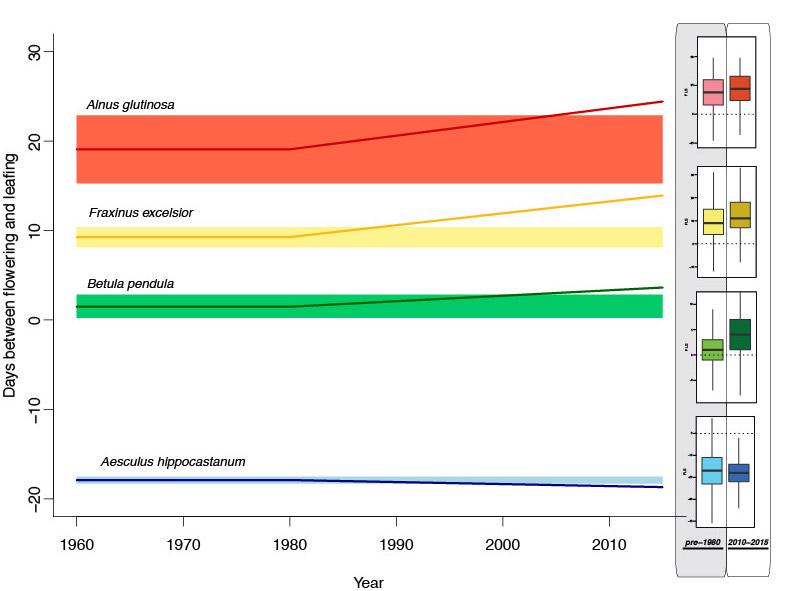
\includegraphics[width=\textwidth]{..//..//PEP725/FLS_climate_change_final.jpg}
    \caption{\textbf{Flower-leaf sequences (FLSs) across Europe for four tree species from 1960 to 2015 suggests climate change has generally increased the time between flowering and leafing}, but the direction and rate of change differs across species, which may exacerbate fitness differences within forest communities. To detect the effect of climate change on average FLSs, we used models that allow for shifts in FLS after 1980 \citep{Kharouba2018}. Lines represent the mean trend in FLS variation per species among populations, and the shaded regions indicate historic range of FLS variability (95\% credible intervals of the pre-1980 average) from the PEP725 database \citep{PEP725}. The boxplots compare the FLS measurements prior to 1980 to the recent period (2010-2015), confirming shifts in FLSs over time for most species, but indicate high variability in the FLSs below the species level. For the boxplots, the middle lines represent median FLS values for each species while the lower and upper hinges of the boxes depict the the 25th and 75th percentiles of the data respectively.}
    \label{fig:climchange}
\end{figure}

\begin{figure}[h!]
    \centering
% 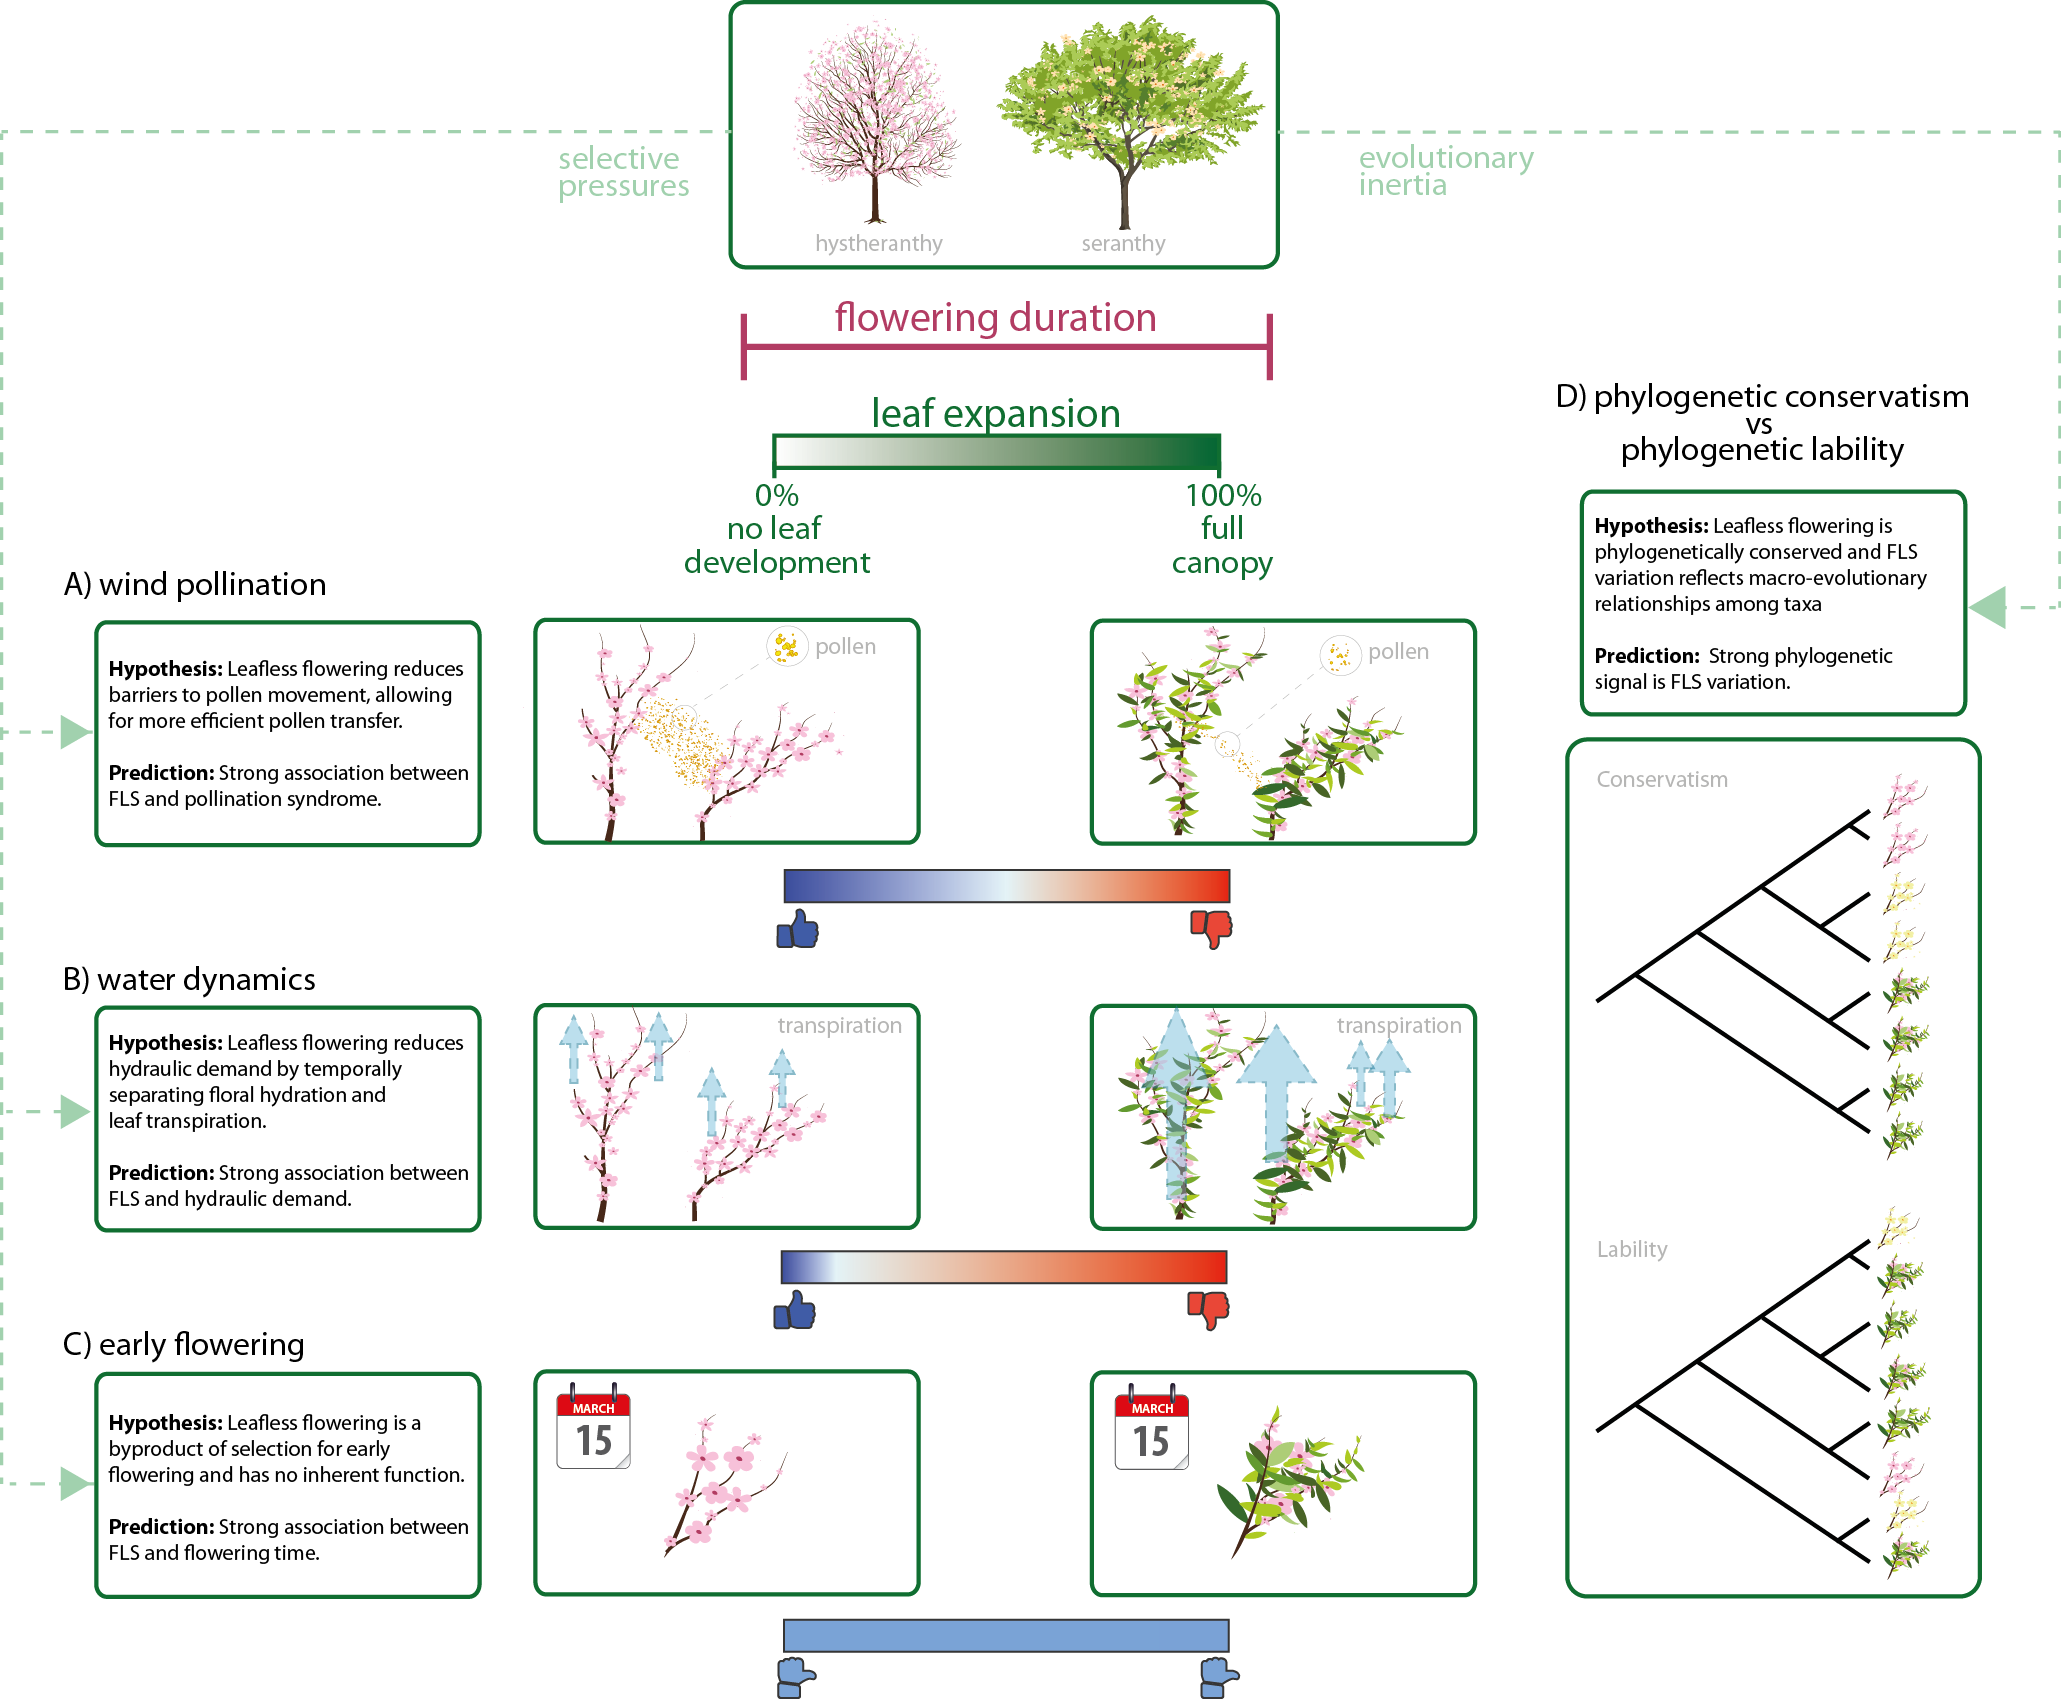
\includegraphics[width=\textwidth]{..//..//HarvardForest/concept_hystheranty_wide_text_overlaps.png}  
    \caption{\textbf{Several hypotheses have been proposed to explain flower-leaf sequence (FLS) variation in temperate, deciduous woody plants.}  The wind pollination hypothesis \textbf{(a)} suggests that leafless flowering reduces barriers to pollen movement. The water limitation hypothesis \textbf{(b)} suggests the temporal separation between flowering and leafing reduces hydraulic demand. The early flowering hypothesis \textbf{(c)} suggests FLS variation is a byproduct of selection for early flowering, possibly driven by later phenological events (e.g., seed dispersal), and under this hypothesis the relative timing of flowers and leaves is inconsequential compared to the absolute time of flowering. As depicted by the scale bars in the center of the figure, the biology behind each hypothesis predicts different degrees of overlap between flowering and leaf development. Transpiration intensifies as small leaf primordia expand, but leaf development only affects environmental structure once leaves are sufficiently large, therefore the water limitation hypothesis accommodates little overlap between flower and leaves, while the wind pollination hypothesis encompasses some overlap. The early flowering hypothesis predicts no fitness differences whether or not flowers and leaves overlap. Additionally, inter-specific patterns of FLS variation may also be a product of phylogenetic conservatism or lability driven by physical constraints. \textbf{(d)}.}
    \label{fig:conceptual}
\end{figure}
  
 \begin{figure}[h!]
        \centering
        % 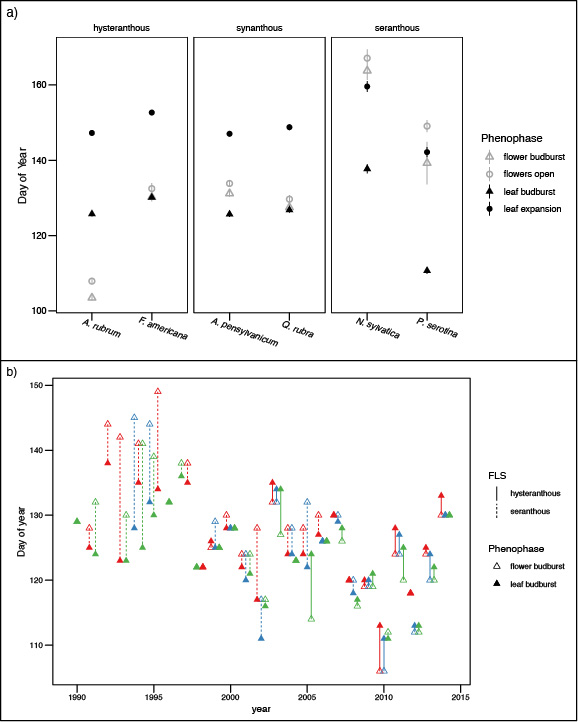
\includegraphics[width=0.8\textwidth]{..//..//intraspecificplots.jpg}
          \caption{\textbf{The shift from categorical/inter-specific descriptions to quantitative/intra-specific measures of flower-leaf sequences (FLSs) reveals substantial variation.} Under the current framework, species are assigned to FLS categories by the order of phenophases alone. However, observations from Harvard Forest in Petersham, MA demonstrate that measuring the time between phenophases reveals substantial differences among species within each category \textbf{(a)}. These records \textbf{(b)} show that the time between flowering and leaf activity can vary significantly among individuals (plotted in different colors) and, within an individual, vary across years. In some species like \emph{Quercus rubra} depicted in here, an individual's sequence itself regularly switches across time. This inter- and intra- specific variation is key to understanding the function of FLS variation in deciduous, woody plants. Data comes from \citet{OKeefe2015}.}
        \label{fig:vizzy}
    \end{figure}

\pagebreak  

 \begin{figure}[h!]
        \centering
        % 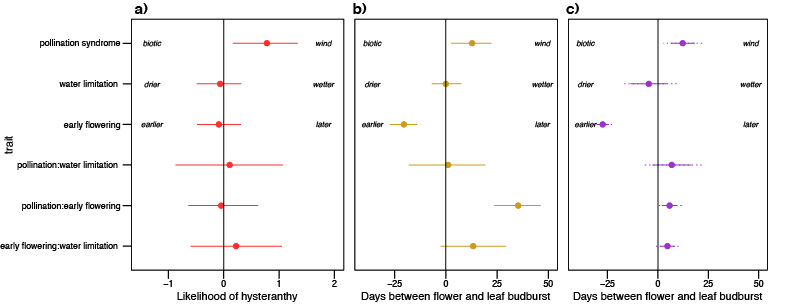
\includegraphics[width=\textwidth]{..//..//HFmodelplots.jpg}
          \caption{\textbf{Mean estimates of the effects of flower-leaf sequence (FLS) predictors on the timing between flower and leaf budburst for woody plants at Harvard Forest between 1990-2015 reveal important differences between categorical and quantitative frameworks of FLSs.}  With the categorical approach in \textbf{(a)}, there is a strong effect of  pollination syndrome on FLS variability, with no detectable effect of other predictors. With quantitative measures based on the species level means of days between flower and leaf budburst in \textbf{(b)}, there are strong effects and interactions of both flowering time and pollination syndrome. Finally, incorporating variation below the species level through hierarchical modeling in \textbf{(c)}, reveals interactions between the predictors. These interactions suggest there are multiple drivers of FLS variability in the temperate zone. All models use standardized predictors to allow for comparisons between them. Symbols represent mean estimated effect of each predictor, with solid lines in \textbf{(a)} and \textbf{(b)} representing the 95\% bootstrap intervals of the phylogenetic linear regression models \citep{Ives2010}. Solid and dotted lines in \textbf{(c)} represent 50 and 95\% credible intervals respectively for a phylogenetic mixed model \citep{Garamszegi2014}. Graphical interpretation of the model interactions of the hierarchical model can be found in the Supporting Information (Fig. \ref{fig:apcs}). The relative sign and magnitude of the estimated effects remained stable in models using alternative functional traits to represent each hypothesis (Supporting Information Fig. \ref{fig:altpreds}).}  
        \label{fig:muplotsHF}
    \end{figure}    


    
\end{document}
